\documentclass[tikz,border=7mm]{standalone}
\usepackage[T1]{fontenc}
\usepackage{xcolor}
\usepackage{amsmath,amssymb}
\usepackage{tikz}
\usetikzlibrary{positioning,arrows.meta,calc,fit,backgrounds,shapes.geometric}

\tikzset{
  flow/.style={-{Stealth[length=2.5mm]}, line width=0.9pt, draw=black!68},
  feedback/.style={-{Stealth[length=2.5mm]}, line width=0.9pt,
    dashed, draw=red!72!black},
  block/.style={draw=black!55, fill=white, rounded corners=3pt,
    minimum height=1.35cm, text width=2.05cm, align=center,
    inner xsep=4pt, font=\small},
  encoder/.style={trapezium, trapezium left angle=82, trapezium right angle=98,
    draw=blue!62!black, fill=blue!9, minimum height=1.55cm,
    text width=1.70cm, align=center, font=\small},
  decoder/.style={trapezium, trapezium left angle=98, trapezium right angle=82,
    draw=green!55!black, fill=green!9, minimum height=1.55cm,
    text width=1.70cm, align=center, font=\small},
  latent/.style={circle, draw=blue!65!black, fill=blue!14,
    minimum size=0.82cm, inner sep=0pt, font=\small},
  peakbox/.style={draw=purple!68!black, fill=purple!8, rounded corners=3pt,
    minimum height=1.05cm, text width=2.15cm, align=center, font=\small},
  outbox/.style={draw=orange!78!black, fill=orange!12, rounded corners=3pt,
    minimum height=1.05cm, text width=1.75cm, align=center, font=\small},
  badge/.style={draw=black!35, fill=black!4, rounded corners=6pt,
    inner xsep=6pt, inner ysep=3pt, font=\scriptsize},
  title/.style={font=\Large\bfseries, anchor=west},
  subtitle/.style={font=\small, text=black!58, anchor=west},
  label/.style={font=\scriptsize, text=black!60, align=center}
}


\begin{document}
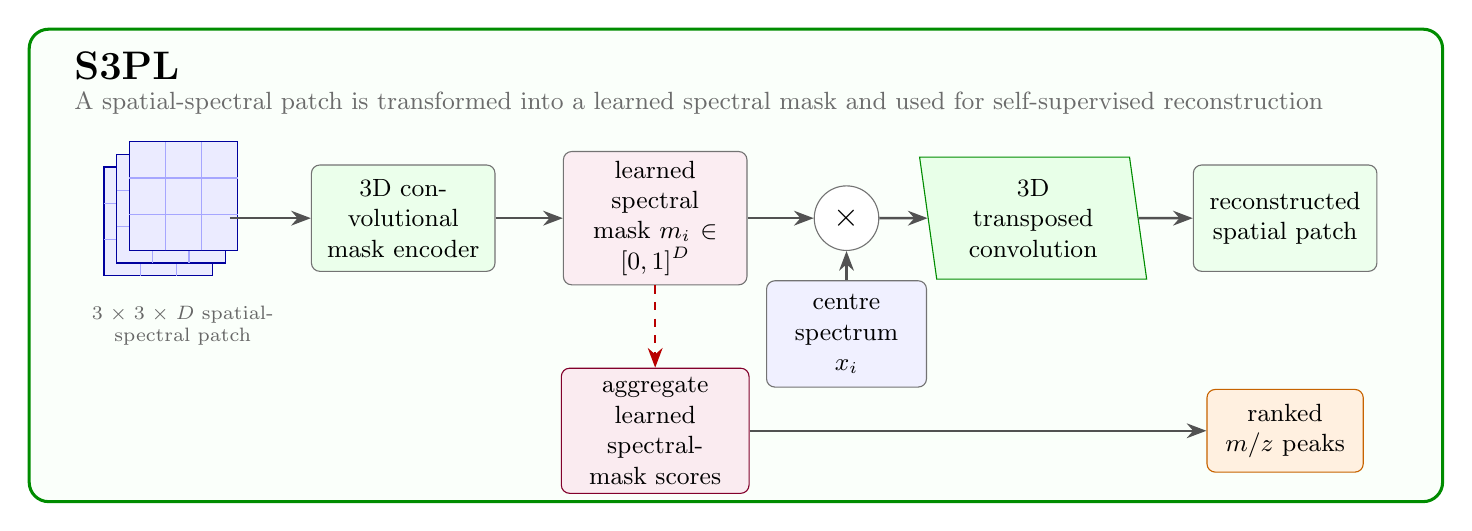
\begin{tikzpicture}[font=\sffamily]
  \fill[green!2, rounded corners=7pt] (-0.6,2.45) rectangle (17.35,-3.55);
  \draw[green!55!black, rounded corners=7pt, line width=1.1pt]
    (-0.6,2.45) rectangle (17.35,-3.55);
  \node[title] at (-0.15,1.98) {S3PL};
  \node[subtitle] at (-0.15,1.51)
    {A spatial-spectral patch is transformed into a learned spectral mask and used for self-supervised reconstruction};

  % Stacked 3D spatial-spectral patch.
  \foreach \k in {0,0.16,0.32}{
    \draw[blue!62!black, fill=blue!8]
      ($(0.35,-0.68)+(\k,\k)$) rectangle ++(1.38,1.38);
    \draw[blue!35] ($(0.35,-0.22)+(\k,\k)$) -- ++(1.38,0);
    \draw[blue!35] ($(0.35,0.24)+(\k,\k)$) -- ++(1.38,0);
    \draw[blue!35] ($(0.81,-0.68)+(\k,\k)$) -- ++(0,1.38);
    \draw[blue!35] ($(1.27,-0.68)+(\k,\k)$) -- ++(0,1.38);
  }
  \node[label, text width=3.1cm] at (1.35,-1.32)
    {$3\times3\times D$ spatial-spectral patch};

  \node[block, fill=green!8] (maskenc) at (4.15,0.05)
    {3D convolutional\\mask encoder};
  \node[block, fill=purple!7] (mask) at (7.35,0.05)
    {learned spectral\\mask $m_i\in[0,1]^D$};
  \node[circle, draw=black!55, fill=white, minimum size=0.82cm,
    inner sep=0pt, font=\large] (times) at (9.78,0.05) {$\times$};
  \node[decoder] (dec) at (12.15,0.05)
    {3D transposed\\convolution};
  \node[block, fill=green!7] (recon) at (15.35,0.05)
    {reconstructed\\spatial patch};
  \draw[flow] (1.95,0.05) -- (maskenc);
  \draw[flow] (maskenc.east) -- (mask.west);
  \draw[flow] (mask.east) -- (times.west);
  \draw[flow] (times.east) -- (dec.west);
  \draw[flow] (dec.east) -- (recon.west);

  \node[block, fill=blue!6, text width=1.75cm] (centre) at (9.78,-1.42)
    {centre spectrum\\$x_i$};
  \draw[flow] (centre) -- (times);

  \node[peakbox] (aggregate) at (7.35,-2.65)
    {aggregate learned\\spectral-mask scores};
  \node[outbox] (peaks) at (15.35,-2.65)
    {ranked\\$m/z$ peaks};
  \draw[feedback] (mask.south) -- (aggregate.north);
  \draw[flow] (aggregate) -- (peaks);
\end{tikzpicture}
\end{document}
